\documentclass[11pt,twoside]{article}
\usepackage{geometry}
\usepackage{enumerate}
\usepackage{latexsym,booktabs}
\usepackage{amsmath,amssymb}
\usepackage{graphicx}
\usepackage{natbib}
\usepackage[singlespacing]{setspace}

\geometry{a4paper,left=3cm,right=2.0cm, top=2cm, bottom=2.0cm}

\newtheorem{Definition}{Definition}
\newtheorem{Theorem}{Theorem}
\newtheorem{Lemma}{Lemma}
\newtheorem{Corollary}{Corollary}
\newtheorem{Proposition}{Proposition}
\newtheorem{Algorithm}{Algorithm}
\numberwithin{Theorem}{section}
\numberwithin{Definition}{section}
\numberwithin{Lemma}{section}
\numberwithin{Algorithm}{section}
\numberwithin{equation}{section}


\begin{document}

\pagestyle{empty}

% =============================================================================
% Title page
% =============================================================================
\begin{titlepage}
\vspace*{.5em}
\center
\textbf{\large{The School of XXXXXX}} \\
\vspace*{1em}
\vspace{2em}
\textbf{\Huge{Scotland Water - XXXXX}}\\[2em]
\textbf{\LARGE{by}}\\
\vspace{2em}
\textbf{\LARGE{XXXX XXXX, 000001}}\\
\vspace{6.5em}
\vspace{6.5em}
\Large{June 2020}\\
\vspace{3em}
\normalsize{Supervised by\\Dr ??? ???}
\vfill
\end{titlepage}

\clearpage

% =============================================================================
% Acknowledgments, and own work declaration
% =============================================================================

% \begin{center}
% \Large{Acknowledgments}
% \end{center}

% Here come your acknowledgments ...

% \clearpage

\begin{center}
\Large{Own Work Declaration}
\end{center}
Here comes your own work declaration

\cleardoublepage



% =============================================================================
% Table of contents, tables, and pictures (if applicable)
% =============================================================================

\tableofcontents
\clearpage

\pagestyle{plain}
\setcounter{page}{1}
\pagenumbering{Roman}

\cleardoublepage

\pagenumbering{arabic}
\setcounter{page}{1}


\clearpage

\section*{Executive summary}
\label{sec.intro}

Here I will write a very good, precise and brief executive summary.
\clearpage

\section{Introduction}
\label{sec.intro}

\clearpage

\section{Background}
\label{sec:background}
Lead has many virtues when it comes to making pipes, water tanks, and
taps because of its low melting point and resistance to corrosion.
Lead, however, is toxic to human beings. update.

\clearpage

\section{Exploratory \& initial data analysis}
\label{sec.explore}

\subsection{Raw data}
\label{sec:raw}



\clearpage

\section{Technical Stuff}

Now it's getting very technical \ldots{} I will cite \cite{shiina} \cite{groewe2001}.

\subsection{Important Things}
Finally we should have a nice picture like this one.
However, I won't forget that figures and table are environments which float around in my document.
So LaTeX will place them wherever it thinks they fit well with the surrounding text.
I can try to change that with a float specifier, e.g..

\begin{figure}[!ht]
\centering
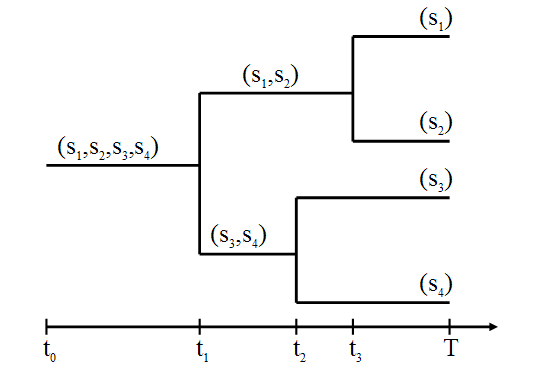
\includegraphics[width=0.5\textwidth]{scenTree.png}
\caption{Look at this scenario tree with funny times $t_{1}$ and scenarios $s_{1}$ etc.}
\label{fig:scenarioTree}
\end{figure}
Now I want to use one of my own environments. I want to define something.

I definitely need some good tables, so I do this.
\begin{table}[!ht]
\centering
\begin{tabular}{|ll|rrrr|}
\hline
Case&Generators&Therm. Units&Lines&Peak load: [MW]&[MVar]\\
\hline\hline
6 bus&3 at 3 buses&2&11&210&210\\
9 bus&3 at 3 buses&3&9&315&115\\
24 bus&33 at 11 buses&26&38&2850&580\\
30 bus&6 at 6 buses&5&41&189.2&107.2\\
39 bus&10 at 10 buses&7&46&6254.2&1387.1\\
57 bus&7 at 7 buses&7&80&1250.8&336.4\\
\hline
\end{tabular}
\caption{Something that doesn't make sense.}
\label{tab:things}
\end{table}
I should really refer to Table \ref{tab:things}.


\section{Conclusions}
I have no idea how to conclude, so I don't write much. But the stuff that follows is important.
\clearpage

% the entries have to be in the file literature.bib
\bibliographystyle{agsm}
\bibliography{literature}
\clearpage

\appendix
\section*{Appendices}
\addcontentsline{toc}{section}{Appendices}

\section{An Appendix}
\label{app:one}

Some stuff.
\clearpage

\section{Another Appendix}
\label{app:two}

Some other stuff.

\end{document}
